\section{External documents: does compiling a wiki help?}
\label{sec:external}
A second, exploratory track uses 118 MIT-licensed development pages from GBrain's externally authored \texttt{messy-company-v1} corpus: one fictional company, eight account histories and 22 supplied questions. The research agent inspected the development labels; this is not a hidden test or independent expert validation. It asks factual retrospective QA, not action choice. The snapshot grants access to all documents, including fictional private-marked notes. It does not test causal observation-time or permission enforcement.

We compile the same raw documents with GPT into a generic company wiki and a wiki organized around marketing decisions. The compiler receives no questions, labels or answer feedback. Both use low reasoning, the same 32,000-token maximum and identical preservation instructions apart from organizational schema. The final wikis contain 66,742 and 63,942 bytes, respectively, versus 293,342 bytes for the rendered raw source packet: reductions of 77.2\% and 78.2\%. These are original, single-pass Markdown compilations inspired by file-memory practice, not an official Karpathy system.\footnote{We inspected the unofficial MIT implementation at \url{https://github.com/Astro-Han/karpathy-llm-wiki}. Karpathy’s owning Gist was inaccessible from this runtime; we do not quote it or claim to execute an official release.} Native asynchronous generation resolves transport limits; previous timed-out and truncated attempts are retained.

\begin{figure}[t]
\centering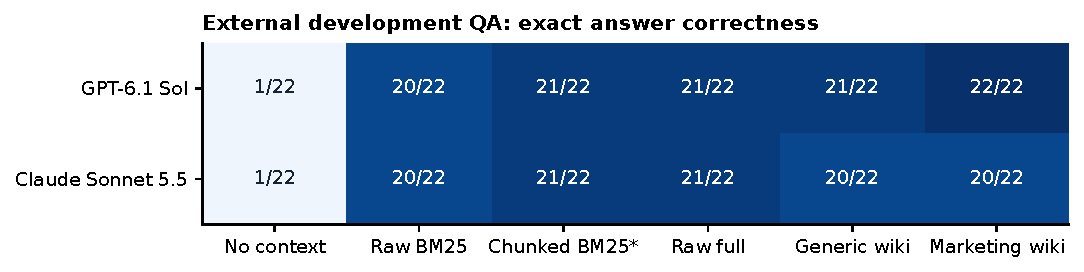
\includegraphics[width=\linewidth]{figures/integrated/external-qa.pdf}
\caption{External development QA, 22 questions per cell. The starred chunked-BM25 control was added after error inspection; all original scores remain. Unequal context lengths, one company and visible development labels prevent a confirmatory specialization claim.}
\label{fig:external}
\end{figure}

Figure~\ref{fig:external} compares no context, whole-document BM25, full raw documents and both compiled wikis with each fixed reader. The marketing wiki scores 22/22 with GPT and 20/22 with Claude; the generic wiki scores 21/22 and 20/22. Full raw context scores 21/22 with both. All 220 original reader calls completed. Every returned citation ID is valid, but this check does not establish that a cited passage entails the answer.

\paragraph{A stronger simple retrieval control.}
Whole-document BM25 scores 20/22 for both readers. Inspection found that the 58,320-byte master agreement could never fit its 24,576-byte allowance, regardless of rank. An explicitly post-hoc 44-call control uses 2,048-character windows with 256-character overlap, the same BM25 and byte allowance, and no label-based filtering. It scores 21/22 for each reader and restores the missing 120-day clause. Chunked BM25 costs \$0.370 for 22 GPT calls and \$0.509 for 22 Claude calls, compared with \$0.905 and \$1.216 for the marketing wiki's reads, before compilation. Thus a wiki's compression relative to full context does not imply an advantage over competent chunked retrieval.

\begin{table}[t]
\centering\small
\begin{tabularx}{\linewidth}{@{}p{.20\linewidth}XX@{}}
\toprule
Observed case & Source/answer diagnosis & Implication \\
\midrule
Notice period & Whole-document retrieval omits a long agreement; both readers correctly say unknown. Chunking recovers the 120-day clause. & An ingestion/packing defect can masquerade as a memory-quality gap. \\
Dated account alias & The raw September 15 update explicitly places ``Dana's freight account'' under Quarrendon. Compiled wikis omit that phrase; Claude misidentifies or withholds. & Preserving entity lists need not preserve a contextual relation. \\
Buyer-role change & March CRM names the CFO; May follow-up distinguishes COO decision maker from budget approver. Claude treats the marketing wiki's preserved claims as unresolved. & Evidence preservation and usable resolution are different; reader behavior matters. \\
Ambiguous reference & July prose mentions a Quarrendon visit, but Dana holds two freight accounts. Upstream requires ``ambiguous''; both full-context readers infer Quarrendon. & One plausible-reference disagreement can determine a small benchmark's ranking. \\
\bottomrule
\end{tabularx}
\caption{Qualitative inspection of observed failures by the same AI-assisted research process, not blinded human review. Source chains and raw explanations are released.}
\label{tab:qualitative}
\end{table}

The last case in Table~\ref{tab:qualitative} is consequential. A disclosed post-hoc sensitivity removes that one question without changing any primary label: GPT's marketing wiki, generic wiki, full context and chunked BM25 all score 21/21. Claude scores 19/21 with the marketing wiki, 20/21 with the generic wiki, and 21/21 with full or chunked raw context. The apparent one-answer GPT advantage is therefore not robust evidence of general marketing-wiki superiority. No wiki is refined in response to these errors.
